Проблема эффективного прогнозирования социально-экономических процессов в
настоящее является исключительно актуальной задачей. Особенную сложность
прогнозирование приобретает в задачах государственного управления. В силу того,
что государственные планы и прогнозы затрагивают жизнь большого числа людей,
возрастает цена ошибки. Поэтому необходимо минимизировать риски. Одним из
способов минимизации рисков является научный подход в прогнозировании возможных
сценариев развития общества.  

Социально-экономическим процессам свойственны неопределенность, наличие скрытых
факторов влияния, слабая предсказуемость. Системы, характеризующиеся такими
процессами, называют нелинейными, хаотическими, случайными, неопределенными.
Существуют математические теории, призванные <<уточнять>> неточности: теория
детерминированного хаоса, теория вероятностей, нечеткая логика и др. В данной
работе рассматриваются прикладные аспекты социального прогнозирования с помощью
нечеткой логики.

\textbf{Цель данной главы:} разработка модели прогнозирования доли
наркозависимых в населении Санкт-Петербурга с помощью индикаторов
наркотизации.%выяснение перспектив применения одномерных нечетких моделей.

\textbf{Поставленные задачи} для достижения цели главы:
\begin{itemize}
    \item опытная проверка результатов одномерных нечетко-логических моделей и
        сравнение с	моделями на основе теории нечетких временных рядов;
    \item опытная оценка результатов многомерных нечетко-логических моделей, 
        задействующих в качестве предикторов социально-экономические показатели.
\end{itemize} 

\section{Вычислительный эксперимент нечеткой авторегрессии}

\subsection{Используемые программные средства}

В настоящей работе программная реализация методов нечеткого прогнозирования
базируется на библиотеке <<frbs>> языка статистического программирования R.
Библиотека разработана докторами философии и аспирантами Гранадского
университета. В библиотеке реализовано более 15 методов нечеткой классификации и
регрессии. В библиотеке рассматриваются системы с многими входами и единым
выходом (MISO) с данными в виде вещественных чисел.

СНВ --- система нечеткого вывода.
\begin{enumerate}
\item СНВ, основанные на разбиении области определения.
\begin{itemize}
\item Метод Ванга и Менделя. Предназначен для решения задач регрессии~\cite{Wang1992}.
\item Метод Чи. Предназначен для решения задач классификации~\cite{Chi1996}.
\item Взвешенный метод Ишибучи. Предназначен для решения задач классификации~\cite{Ishibuchi2001}.
\end{itemize}
\item СНВ, основанные на искусственных нейронных сетях.
\begin{itemize}
	\item Адаптивная нечеткая система вывода с использованием нейросети. Предназначена для решения задач регрессии~\cite{Jan1993}. 
	\item Гибридная нечеткая система вывода с использованием нейросети.  Предназначена для решения задач регрессии~\cite{Kim1999}.
\end{itemize}
\item СНВ, основанные на алгоритмах кластеризации.
\begin{itemize}
	\item Субтрактивная кластеризация и метод нечеткой кластеризации c-средних.
	Предназначена для решения задач регрессии~\cite{Chiu1996}.
	\item Динамическая эволюционирующая система вывода с использованием нейросети. Предназначена для решения задач регрессии~\cite{Kasabov2002}.
\end{itemize}	
\item СНВ, основанные на генетических алгоритмах.
\begin{itemize}
	\item Метод Трифта. Предназначен для решения задач регрессии~\cite{Thrift1991}.
	\item Генетическая нечеткая система для обучения нечетких правил, основанная на технологии MOGUL. Предназначен для решения задач регрессии~\cite{Cordon1999}.
	\item Метод Ишибучи, основанный на генетическом кооперативно-кон\-курентном обучении. Предназначен для решения задач классификации~\cite{Ishibuchi1999}.
	\item Метод Ишибучи, основанный на гибридизации генетического ко\-оперативно-конкурентного обучения и Питтсбургского метода. 
	 Предназначен для решения задач классификации~\cite{Ishibuchi2005}.
	\item Структурный обучающий алгоритм на нечеткой среде.  
	Предназначен для решения задач классификации~\cite{Gonzalez2001}. 
	\item Генетический алгоритм для латеральной настройки и выбора правил лингвистической нечеткой системы. 
	Предназначен для решения задач регрессии~\cite{Alcala2007}.
\end{itemize}
\item СНВ, основанные на методе градиентного спуска.
\begin{itemize}
	\item СНВ с использованием эвристик и градиентного спуска. Предназначена для решения задач регрессии~\cite{Ishibuchi1994}.
	\item Правила нечеткого вывода по методу спуска. 
	Предназначен для решения задач регрессии~\cite{Nomura1992}. 
\end{itemize}
\end{enumerate}

\subsection{Методика проведения эксперимента}

Основными направлениями нечеткого прогнозного моделирования, описанными в
литературе, являются теория нечеткой логики~\cite{Zadeh1973} и теория нечетких
временных рядов~\cite{Song1993}.  При этом, для прогнозирования по методу
нечетких временных рядов исследователям удалось добиться существенного снижения
погрешности прогнозов даже для авторегрессионного случая. 

Известно~\cite{sep-principia-mathematica}, что до некоторых пределов математика
сводима к логике. Это и будет исходной точкой нашего эксперимента. Попробуем
сравнить доказанные в своей успешности методы теории нечетких временных рядов
(основанные на математической теории нечетких множеств) с методами нечеткой
логики, реализованными в пакете <<frbs>>.  

Объектом прогнозирования являются данные по поступившим в университет Алабамы абитуриентам за период 1971-1992 гг. (рис.~\ref{figure:UA_enrollments}). Именно они были использованы в статье, впервые описавшей теорию нечетких временных рядов и с тех пор являются основой для сравнения моделей.  

\begin{figure}[bhtp]
    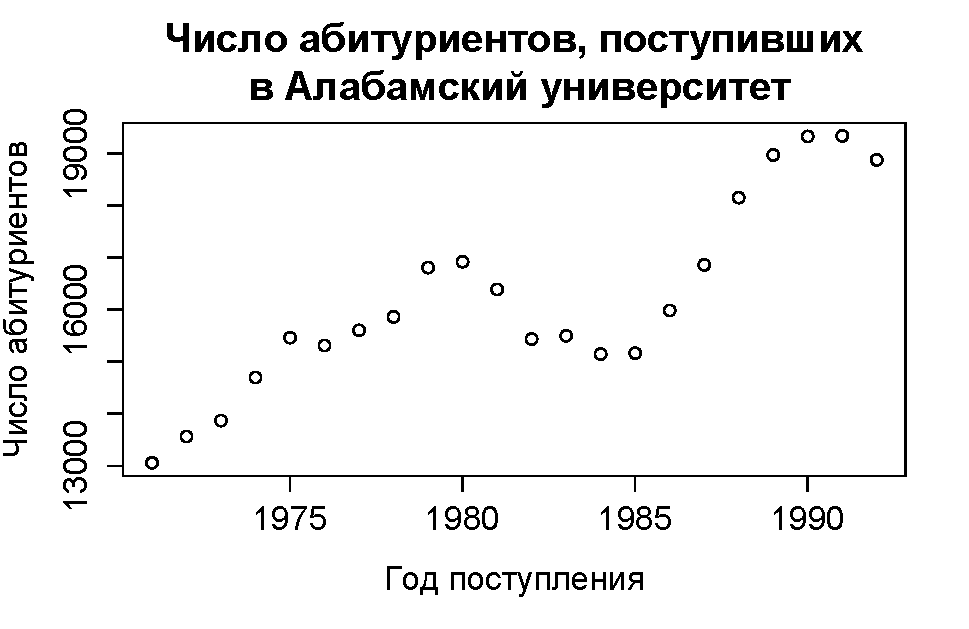
\includegraphics{images/UA_enrollments.pdf}
    \caption{Число поступивших в Алабамский университет, 1971-1992}		
    \label{figure:UA_enrollments}
\end{figure}

По итогам экспресс-теста регрессионных моделей решено было выбрать модель
авторов Л-Х. Ванга и Дж. М. Менделя, основанную на разбиении области
определения~\cite{Wang1992}. Критериями отбора были точность прогноза на
тестовых данных и сложность вычислений. Модель демонстрирует хорошую точность и
низкую вычислительную сложность. 

Алгоритм Ванга и Менделя состоит из пяти шагов:
\begin{enumerate}
	\item Разбиение областей определения входных и выходных численных данных на нечеткие интервалы.
	\item Генерация нечетких правил на основе предоставленных данных.
	\item Присвоение степени каждому из сгенерированных правил с целью разрешения противоречий между правилами.
	\item Создание комбинированной нечеткой базы правил, основанной одновременно на 1) автоматически сгенерированных правилах и
	   2) правилах на естественном языке, предложенных экспертами.
	
	\item Определение отображения входного пространства на выходное, основываясь на комбинированной базе правил, с помощью процедуры дефаззификации.
\end{enumerate}

\begin{table}[bhtp]
	\caption{Пример нечетких правил}
		\begin{tabular}{ | c | c | }
			\hline
			1 & IF tminus2 is  v.1\_a.1 and tminus1 is  v.2\_a.1 THEN   t  is  c.1 \\
			\hline
			2 & IF tminus2 is  v.1\_a.7 and tminus1 is  v.2\_a.7 THEN   t  is  c.5  \\
			\hline
			\multicolumn{2}{ |c| }{\ldots} \\
			\hline
			17 & IF tminus2 is  v.1\_a.9 and tminus1 is  v.2\_a.6 THEN   t  is  c.7 \\
			\hline
		\end{tabular}		
	\label{table:fuzzy_rules_example}	
\end{table}

Доказана возможность предлагаемого отображения аппроксимировать любую
непрерывную функцию вещественного переменного на компактном множестве с
произвольной точностью.  Примеры нечетких правил и функций принадлежности,
генерируемых моделью, приведены на табл.~\ref{table:fuzzy_rules_example} и
рис.~\ref{figure:MFexample}, соответственно.  

\renewcommand{\arraystretch}{1.5} %Space between rows
\setlength{\tabcolsep}{8pt} %Space between columns

\begin{figure}[bhtp]
    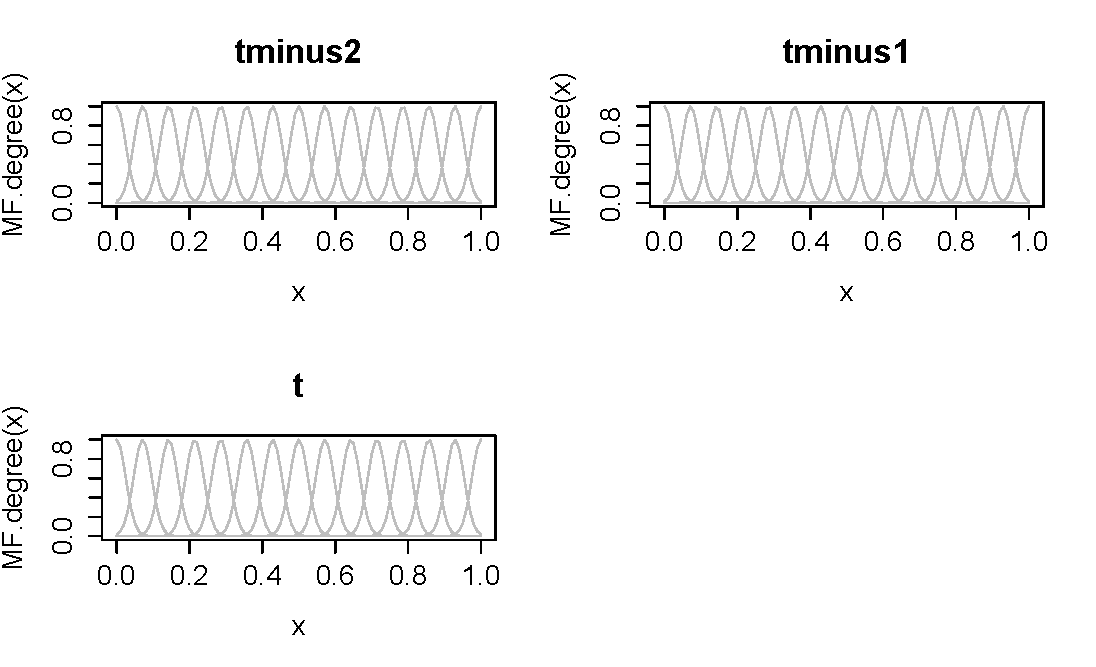
\includegraphics{images/MFexample.pdf}
    \caption{Пример функций принадлежности для лингвистических переменных}		
    \label{figure:MFexample}
\end{figure}

На выходе модели --- численность поступивших в университет Алабамы за период 1971-1992 гг. ($t$). На входе --- эта же переменная, но со сдвигом на один ($tminus1$) и два ($tminus2$) года назад, соответственно. Таким образом реализована импровизированная авторегрессия по переменной $t$. 

Аналогичным образом в тестовых примерах библиотеки <<frbs>> прогнозировались хаотические временные ряды Маки-Гласса, при этом, однако, сдвиг происходил на 4 и 8 позиций назад и общее число наблюдений составляло 300, а не 22, как в случае с временным рядом поступивших в университет Алабамы.

Общее множество данных разбивалось на два подмножества --- данные для обучения модели и данные для сравнения результатов работы модели --- в зависимости от величины горизонта прогнозирования. 

\subsection{Результаты эксперимента}

В эксперименте использовались два значения горизонта прогнозирования --- 5 лет (рис.~\ref{figure:UA_model_h=5}) и 3 года (рис.~\ref{figure:UA_model_h=3}). Заметим, что в обоих случаях симуляция в области данных для обучения сработала достаточно хорошо, несмотря на крайне малый объем выборки. 

\begin{figure}[bhtp]
    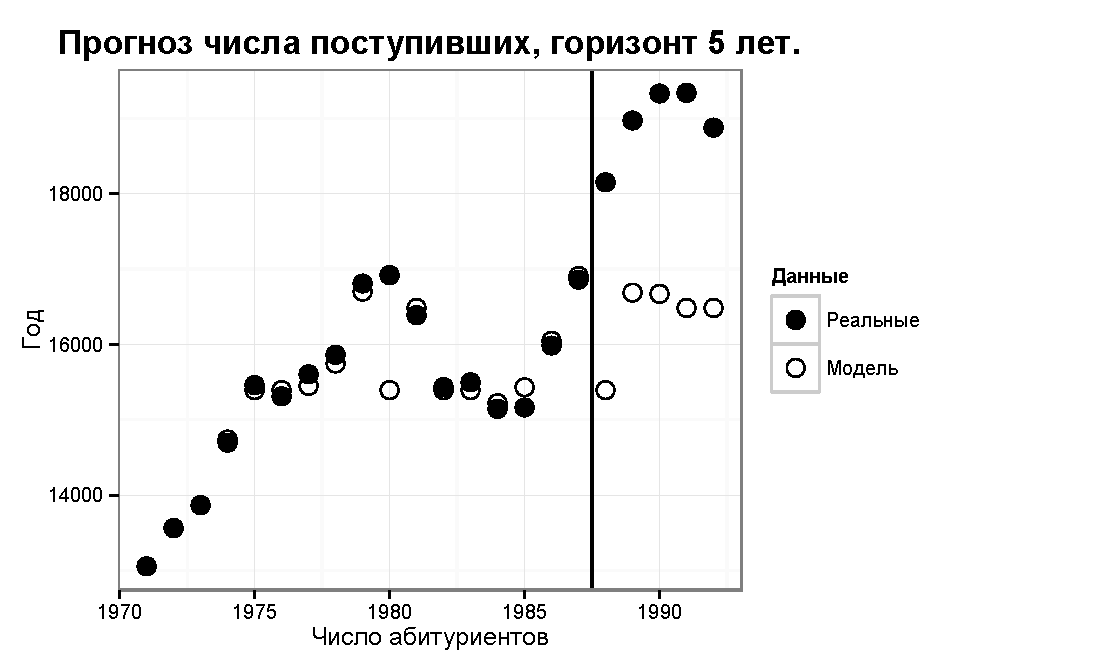
\includegraphics{images/UA_model_h=5.pdf}
    \caption{Прогноз числа поступивших в Алабамский университет, \newline горизонт 5 лет}		
    \label{figure:UA_model_h=5}
\end{figure}

\begin{figure}[bhtp]
    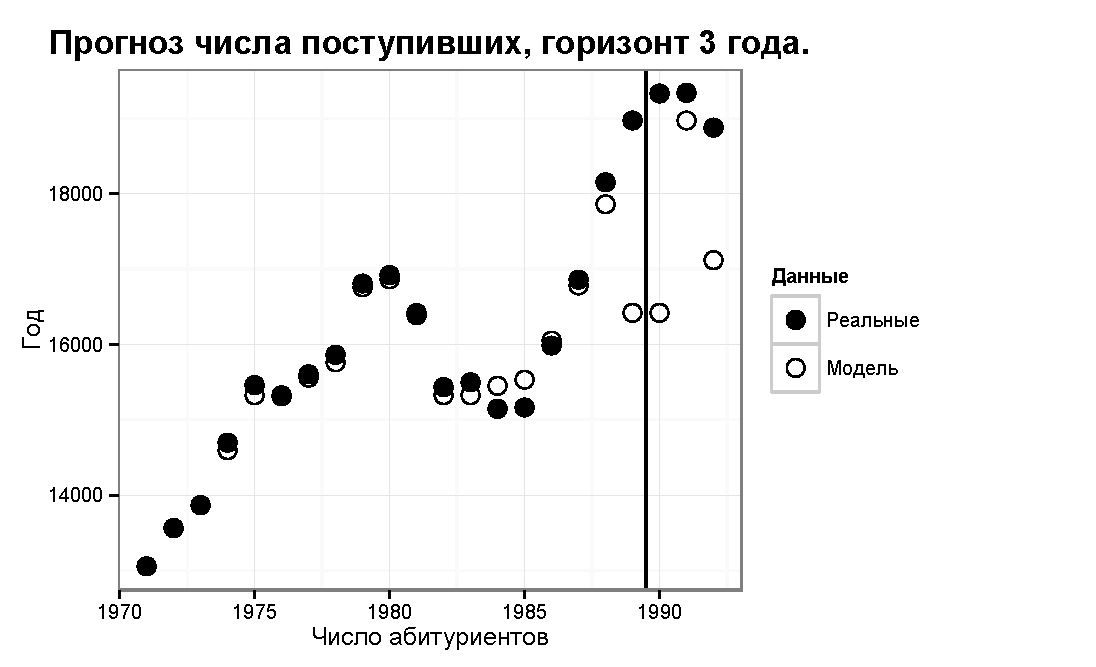
\includegraphics{images/UA_model_h=3.pdf}
    \caption{Прогноз числа поступивших в Алабамский университет, \newline горизонт 3 года}		
    \label{figure:UA_model_h=3}
\end{figure}

В части прогноза же результаты неудовлетворительные. Это подтверждается и оценкой погрешности прогнозирования (табл.~\ref{table:WM-error}). Погрешность гораздо выше, чем при авторегрессии методами нечетких временных рядов. С другой стороны, точность увеличивается при уменьшении горизонта прогнозирования. Это говорит о том, что модель адаптируется при изменении параметров и входных данных. 

\begin{table}[bhtp]
	\caption{Оценка точности результатов прогнозирования}
    \begin{tabular}{ | c | c | c | c | }
        \hline
        Горизонт & MSE & RMSE & SMAPE \\
        \hline
        5 & 6.750612e+06 & 2.598194e+03 & 3.674307e+00  \\
        \hline
        3 & 3.897863e+06 & 1.974301e+03 & 2.330708e+00  \\
        \hline
    \end{tabular}		
	\label{table:WM-error}	
\end{table}

Основной причиной низкой точности прогноза, по нашему предположению, является недостаточность исходных данных. Расширение доступной для модели информации с целью повышения качества прогноза может происходить по трем направлениям:
\begin{itemize}
	\item Увеличение объема выборки (периода, который охватывает временной ряд).
	\item Увеличение количества продукционных правил либо изменение существующих правил.
	\item Увеличение количества либо изменение структуры входных показателей, отбор наиболее релевантных задаче показателей.
\end{itemize}

В процессе вычислительного эксперимента автор столкнулся с техническими трудностями:
\begin{itemize}
	\item Невозможность оценки всех моделей из библиотеки <<frbs>> с варьированием всех параметров моделей ввиду нехватки вычислительных мощностей.
	\item Сложность доступа к данным.  
\end{itemize}
	

\section{Разработка модели прогнозирования численности наркозависимых в 
    Санкт-Петербурге на основе нечеткой модели с многими переменными}

В связи с расширением масштабов незаконного оборота и немедицинского потребления 
наркотиков  в России и в ответ на усиление таких негативных тенденций, связанных 
с наркоситуацией, как устойчивое сокращение численности населения России, в том 
числе уменьшение численности молодого трудоспособного населения, была принята 
Стратегия государственной антинаркотической политики
Российской Федерации до 2020 года~\cite{ru_nat_drug_strat}. 

В качестве генеральной цели Стратегии постулируется <<существенное сокращение 
незаконного распространения и немедицинского потребления наркотиков>>. Таким 
образом, можно утверждать, что Российская Федерации придерживается 
преимущественно политики снижения потребления. Это и будет предпосылкой к 
дальнейшим положениям.

\subsection{Теоретико-методологические основы анализа наркоситуации}

По мнению теоретиков анализа наркоситуации~\cite{Karpets2010}, с позиций
социального управления приобщение части населения к употреблению психоактивных
веществ целесообразно рассматривать как риск. С точки зрения управления, риск
–-- это событие или группа однородных случайных событий, которому присущи два
основных свойства --– вероятность и ущерб.

Вероятность –-- признак, означающий возможность с той или иной степенью точности
рассчитать и прогнозировать частоту наступления неблагоприятного события (в
данном случае --– акта потребления наркотиков) при наличии достаточного
количества данных и результатов наблюдений. Вместе с тем для риска всегда
характерна случайность, непредсказуемость наступления события, означающая
невозможность точно определить время и место его возникновения. А поскольку риск
выбора потребления наркотиков в современном российском обществе сохраняется, то,
с позиций социального управления, управление антинаркотической деятельностью, а
через него –-- и организация влияния на наркоситуацию и контроля за
проявляющимися в ее рамках тенденциями –-- это прежде всего управление рисками.

Одним из важнейших вопросов исследования наркоситуации выступает анализ и
оценка факторов риска, прямо или косвенно влияющих на тенденции наркотизации. 
Факторы риска можно разделить на две группы:
\begin{enumerate}
    \item факторы, имманентно присущие субъекту наркотизации:
        \begin{itemize}
            \item наследственные
            \item гендер
            \item возраст
            \item социальный статус
            \item социокультурные факторы
        \end{itemize}
    \item внешние факторы:
        \begin{itemize}
            \item доступность наркотических и иных психоактивных веществ
            \item информационные факторы	
        \end{itemize}
\end{enumerate}	

Помимо непосредственно факторов наркотизации для анализа 
целесообразно рассмотреть \textbf{индикаторы воздействия}, т.е. статистические 
и эпидемиологические показатели, отражающие криминальную ситуацию, социальное 
положение и состояние здоровья населения.  Основными индикаторами воздействия 
определены следующие:
\begin{enumerate}		
    \item Социально-демографические и экономические:
    \begin{itemize}
        \item число и доля лиц, попробовавших наркотики хотя бы раз в жизни;
        \item процент лиц определенной возрастной группы, употребляющих наркотики;
        \item спрос на наркотики среди населения;
        \item спектр употребляемых наркотиков;
        \item средняя продолжительность и качество жизни населения;
        \item сумма социально-экономического ущерба от наркотиков (социальная 
            стоимость употребления наркотиков).
    \end{itemize}
    \item Медицинские:
    \begin{itemize}
        \item заболеваемость наркоманией;
        \item количество отравлений наркотиками;
        \item процент лиц определенной возрастной группы, зависимых от наркотиков;
        \item смертность, связанная с наркотиками;
        \item доля повторных обращений в медицинскую службу больных наркоманией;
        \item продолжительность и качество жизни лиц, употребляющих наркотики;
        \item распространенность ВИЧ и гепатитов среди потребителей наркотиков.
    \end{itemize}
	
    \item Криминальные:
    \begin{itemize}
        \item число задержанных правоохранительными органами лиц с положительным 
            результатом освидетельствования на состояние наркотической интоксикации;
        \item индикатор доступности наркотиков среди населения;
        \item число и доля лиц, осужденных за преступления, связанные с наркотиками;
        \item рецидивная преступность, связанная с наркотиками.
    \end{itemize}
\end{enumerate}
	
Не все перечисленные выше индикаторы, необходимые для полноценного и 
качественного мониторинга наркоситуации, собираются статистическими службами 
и используются при проведении практических исследований, однако, попытаемся 
оценить эффективность прогнозирования наркоситуации с помощью той их части, 
которая доступна для исследования.

\subsection{Использование индикаторов мониторинга наркоситуации для 
    прогнозирования доли наркозависимых в населении Санкт-Петербурга}

Из числа доступных для анализа показателей, хранящихся в Интегрированной системе 
информационно-аналитического обеспечения деятельности исполнительных органов 
государственной власти Санкт-Петербурга, были отобраны три комбинации для 
составления мультифакторного прогноза показателя <<Состоит на учете больных с 
диагнозом «наркомания», на 100 тыс. населения>>, который, на наш взгляд, 
отражает критерии выполнения задач Стратегии антинаркотической политики в 
области снижения потребления.

\begin{table}[bhtp]
    \caption{Оценка точности результатов прогнозирования}
    \begin{tabular}{ | c | c | c | c | }
        \hline
        № набора & MSE & RMSE & SMAPE \\
        \hline
        (1-мерный) & 6.750612e+06 & 2.598194e+03 & 3.674307e+00  \\
        \hline
        1 & 1099 & 33.14 & 3.733  \\
        \hline
        2 & 6460 & 80.38 & 11.14  \\
        \hline
        3 & 9805 & 99.02 & 14.44  \\
        \hline
    \end{tabular}		
    \label{table:WM-error-multi}	
\end{table}

\begin{itemize}
    \item Набор показателей №1. Независимые переменные:
    \begin{itemize}
        \item Численность безработных, всего;
        \item Преступления связанные с незаконным оборотом наркотиков, 
            зарегистрировано;
        \item Состоит на учете больных с диагнозом «наркомания», на 100 тыс. 
            населения (ретроспективные данные).
    \end{itemize}
    \item Набор показателей №2. Независимые переменные:
    \begin{itemize}
        \item В состоянии наркотического опьянения;
        \item Число отравлений наркотическими веществами, Всего, Все население 
            от 0 до 99 лет  всего;
        \item Состоит на учете больных с диагнозом «наркомания», на 100 тыс. 
            населения (ретроспективные данные).
    \end{itemize}
    \item Набор показателей №3. Независимые переменные:
    \begin{itemize}
        \item Число лиц, осужденных за (ст. 228-233 УК РФ), возрастная структура 
            осужденных  14-17 лет;
        \item Число лиц, осужденных за (ст. 228-233 УК РФ), возрастная структура 
            осужденных  18-24 лет;
        \item Состоит на учете больных с диагнозом «наркомания», на 100 тыс. 
            населения (ретроспективные данные).
    \end{itemize}			
\end{itemize}

\begin{figure}[bhtp]
    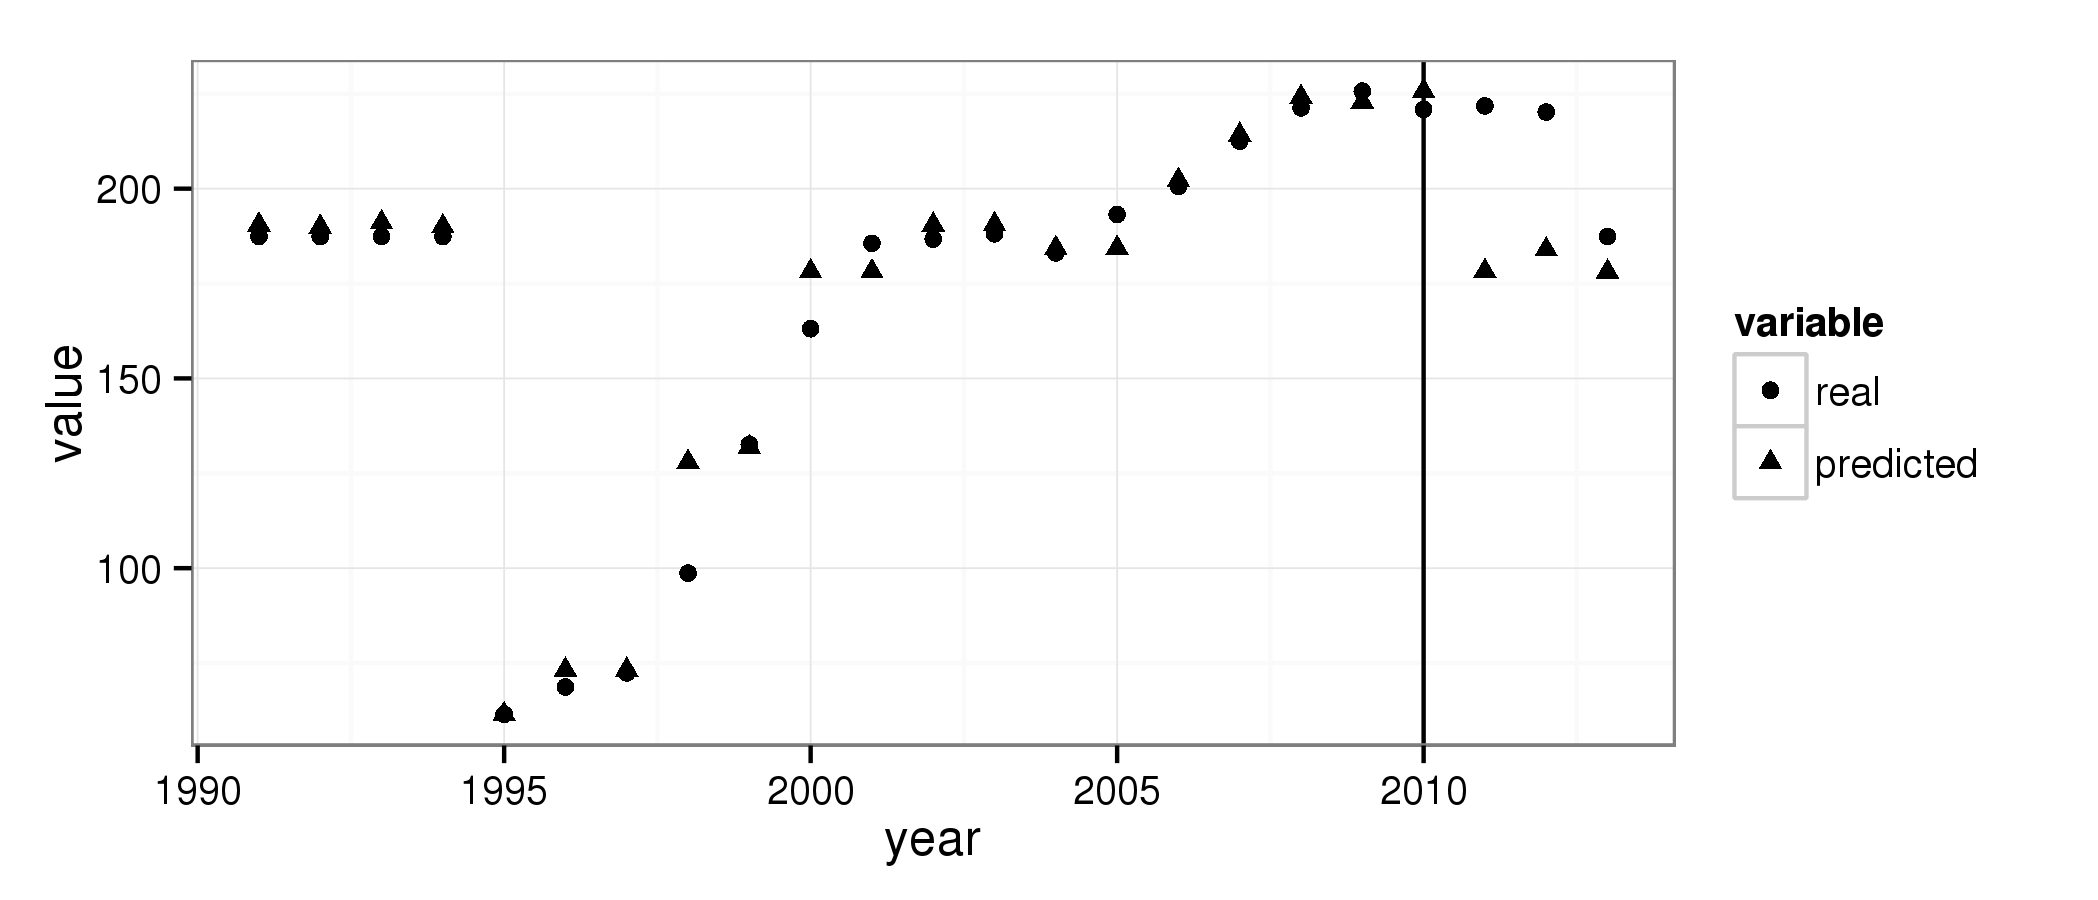
\includegraphics{images/m_plot1.png}
    \caption{Прогноз с набором показателей №1, горизонт 3 года}		
    \label{figure:m_plot1}
\end{figure}

\begin{figure}[bhtp]
    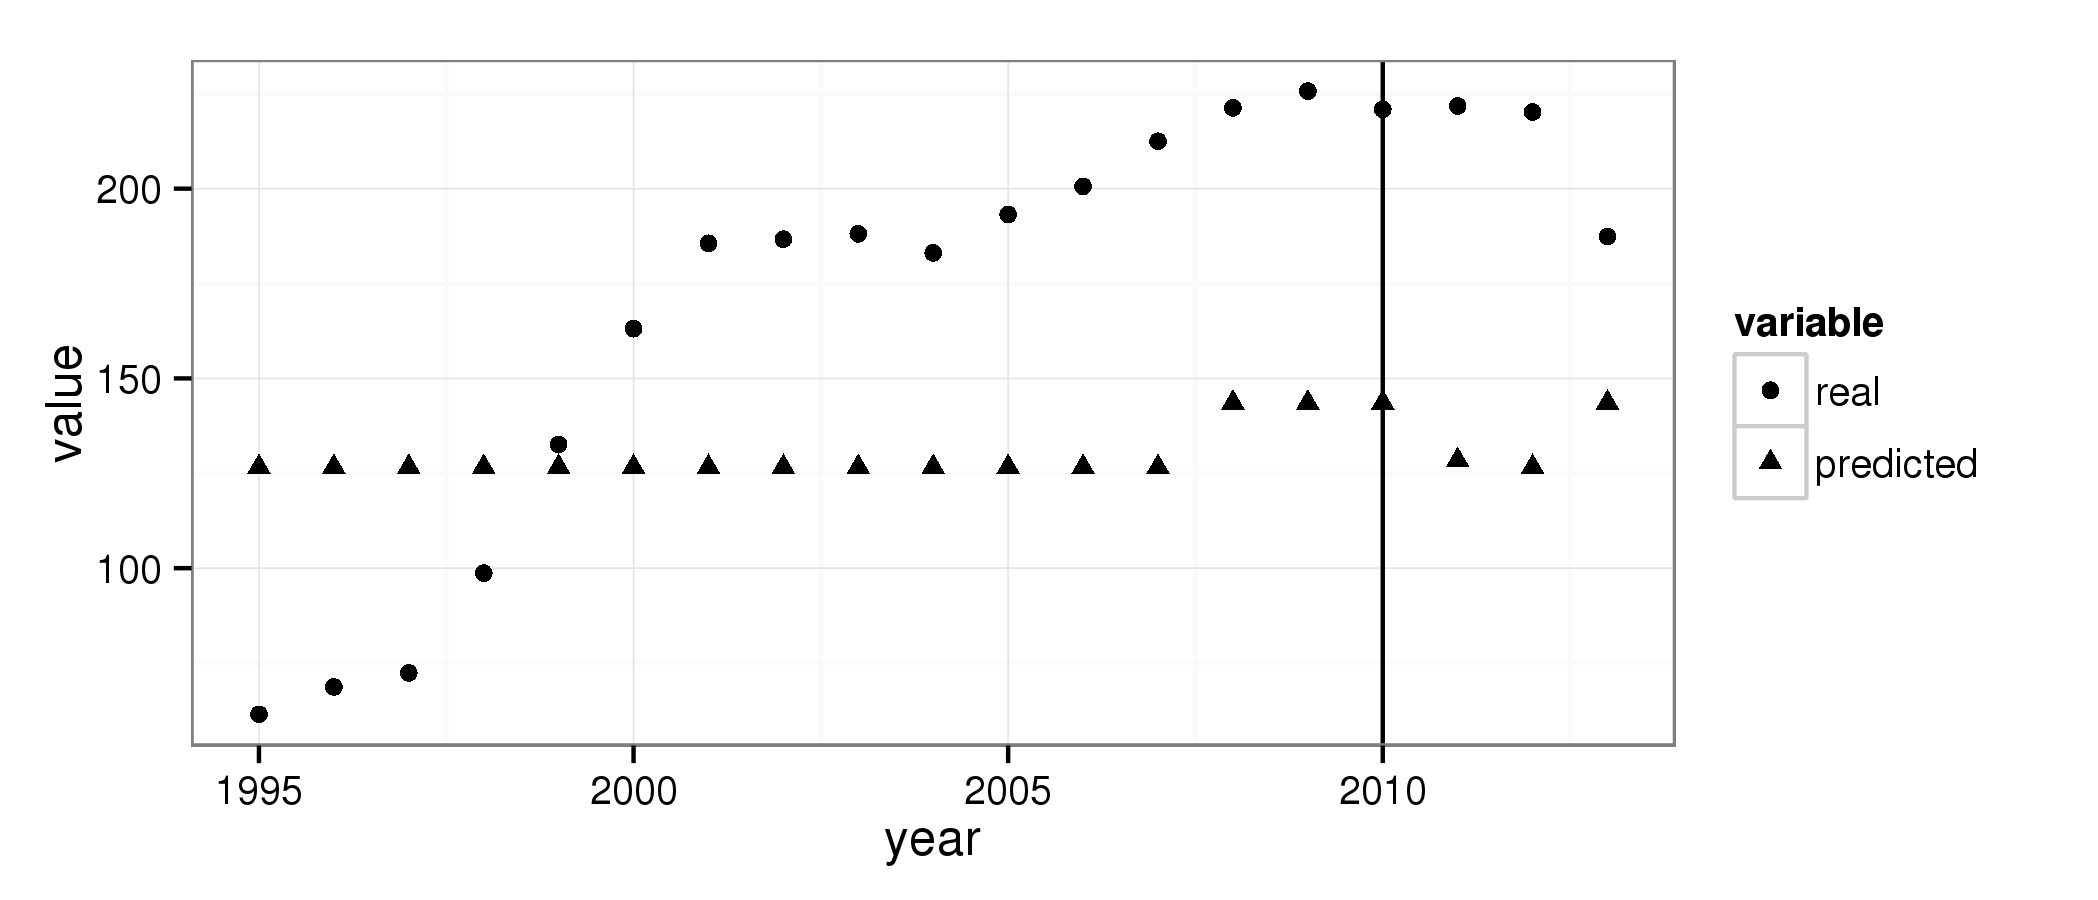
\includegraphics{images/m_plot2.png}
    \caption{Прогноз с набором показателей №2, горизонт 3 года}		
    \label{figure:m_plot2}
\end{figure}

\begin{figure}[bhtp]
    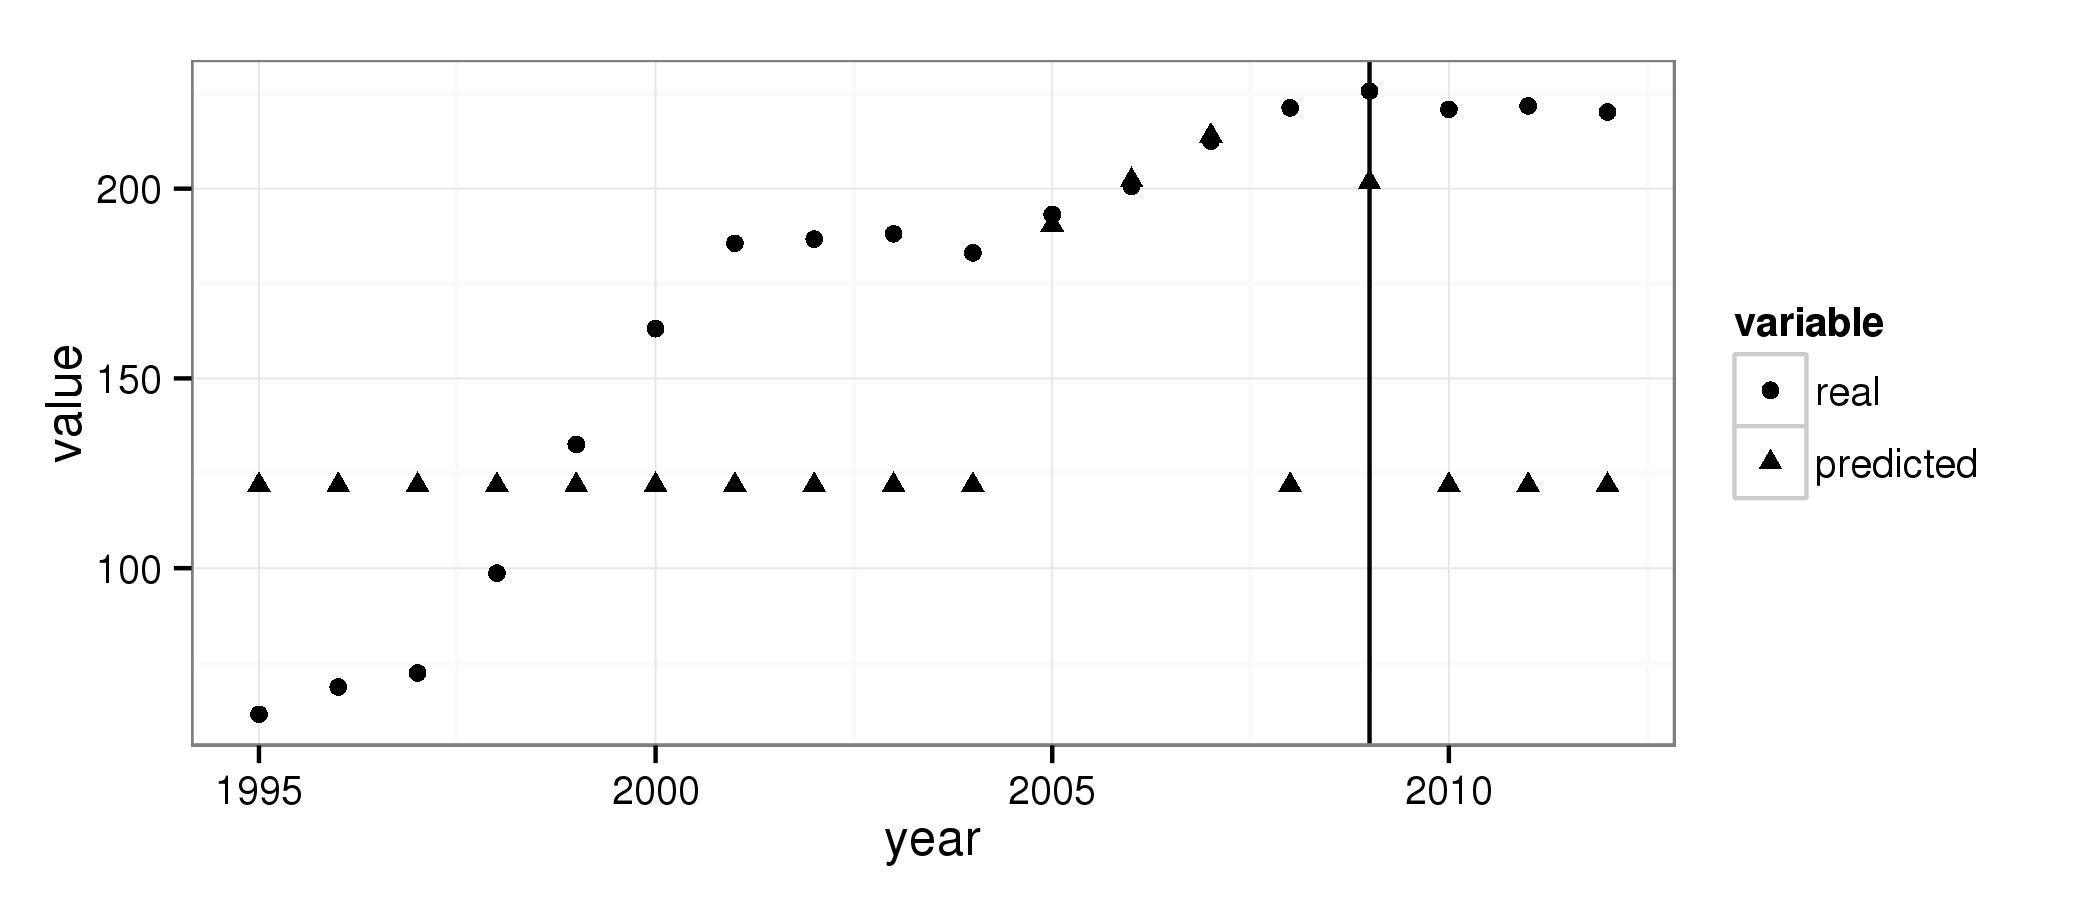
\includegraphics{images/m_plot3.png}
    \caption{Прогноз с набором показателей №3, горизонт 3 года}		
    \label{figure:m_plot3}
\end{figure}

С точки зрения точности прогноза, при использовании набора показателей №1
наблюдается существенное улучшение относительно одномерного варианта.  Однако,
требуемый уровень точности на данный момент не достигнут.

Низкие оценки точности прогноза при использовании наборов показателей №2 и №3
объясняются, по мнению автора, неполнотой исходных данных, которая выражается в
наличии пропущенных значений в независимых переменных, требующих их
экстраполяции (в нашем случае для заполнения пропусков использовалась функция
медианы), что заведомо снижает количество доступной для модели информации, и
искажает характеристики случайных величин, тем самым нарушая механизмы
прогнозирования.

\section{Формальное описание модели}
Предлагаемая модель прогнозирования численности наркозависимых на основе
нечеткой логики состоит из ряда последовательных аналитических шагов:
\begin{enumerate}
    \item Определение исходных данных;
    \item Заполнение пропусков в исходных данных (imputation);
    \item Выбор горизонта прогнозирования;
    \item Обучение модели с помощью алгоритма нечетко-логического вывода;
    \item Получение результатов модели (численных значений временных рядов,
        оценок ошибки прогнозирования, связей между переменными и др.);
    \item Интерпретация результатов модели.
\end{enumerate}
Остановимся на некоторых из данных шагов подробнее. 

\textit{Определение исходных данных.} Модель относится к категории моделей с
множеством входных переменных и одной выходной переменной (MISO). Это означает,
что прежде всего определиться с целевой переменной, прогнозирование которой и
будет осуществляться. В нашем случае, это показатель <<Состоит на учете больных
с диагнозом ``наркомания", на 100 тыс. населения>>, полученный из Информационной
системы информационно-аналитического обеспечения органов государственной власти
Санкт-Петербурга. Однако, в <<сыром>> виде использовать показатели оценки
наркоситуации не эффективно, т.к. ситуация, наблюдаемая органами государственной
статистики и объективная ситуация, как правило, расходятся на несколько порядков
ввиду нелегальной природы самого феномена наркотизма, наркорынков и пр. Для
объективной оценки феномена наркотизации вводится понятие коэффициента
латентности~\cite{Zakharov2012}, определяемого как отношение фактического
значения исследуемой величины (в нашем случае --- числа наркозависимых) к
наблюдаемому значению.  Оценка коэффициента латентности выходит за рамки данного
исследования, добавим лишь, что как правило латентный анализ используется  в
сопряжении с установкой и анализом пороговых уровней, позволяющих судить о
степени кризисности ситуации в зависимости от принадлежности тех или иных
целевых величин соответствующим уровням. Кроме того, для приведения модели к
стандартизированному виду, возможности её сопоставления с аналогами из Банка
моделей и для внедрения элементов вероятностного моделирования целесообразно
переводить абсолютные значения исследуемой величины в вероятность или долю (в
нашем случае --- вероятность заболевания наркозависимостью для отдельно взятого
человека). Таким образом, общая формула манипуляций, производимых с исследуемой
переменной до непосредственно процесса прогнозирования выглядит следующим
образом:
\begin{equation}
    p_{addiction} = \frac{\rho_{drug}}{\rho_{population}}\cdot k
\end{equation}

Где \(p_{addiction}\) --- вероятность заболевания наркозависимостью для отдельно
взятого человека, \(\rho_{drug}\) --- численность наркозависимых по данным
официальной статистики, \(\rho_{population}\) --- численность населения города
Санкт-Петербурга, \(k\) --- коэффициент латентности.

Далее необходимо определиться с составом входных переменных. Модель базируется
на предположении о существовании явной или неявной связи между входными
переменными и выходной переменной. Социальные процессы не связаны такими же
жесткими законами, как физические процессы, но можно предложить методы подбора
входных переменных, способных обеспечить максимальную точность прогнозирования.
К таким методам можно отнести: использование экспертного знания (исследований,
опросов, метода коллегиальной оценки, гипотез и др.), обращение к аппарату
теоретико-методологических основ в исследуемой предметной области, проведение
корреляционного анализа. Помимо этого, модель, в силу своей универсальности,
прдполагает возможность проведения сценарного анализа для учета влияния не
только наркоспецифических, но и общеэкономических и социальных факторов для
обнаружения и потенциального устранения непредвиденного влияния изменений в
какой-либо из сфер жизнедеятельности города на состояние наркоситуации.

\textit{Заполнение пропусков в исходных данных.} Основой моделирования
наркоситуации являются данные государственной статистики.  Однако, на практике,
данные статистических служб имеют свои особенности и ограничения, которые
необходимо учитывать при моделировании. К ним относятся: изменение год от года
методик сбора данных, наличие переходных периодов, когда данные не собираются,
разная частота и периодичность сбора данных в зависимости от конкретных
показателей. Это приводит к неоднородности исходных данных, необходимости их
приведения к нормализованному виду для дальнейшего анализа.  Необходимость
решения данной задачи обусловлена ещё и тем, что зачастую требуется использовать
максимально длинный временной ряд ввиду того, что точность моделей на основе
алгоритмов машинного обучения прямо пропорциональна объему доступной для
обучения информации. И если взять за основу максимально длинный временной ряд,
неизбежно возникают пропуски в случаях его совместного использования с
сопутствующими временными рядами.  Для решения этой задачи используются методы
т.н. <<imputation>> или заполнения пропусков в данных. К таким методам относятся
функции агрегирования (например, месячные, годовые средние, медианы и т.п.),
аппроксимирования (интерполяции, сплайны и др.), метод LOCF (<<последнее
наблюдаемое значение переносится вперёд>>), фильтры (например, сезонный фильтр
Калмана), наконец, ручное заполнение пропущенных значений и обрезание
пропущенных значений в конце и начале временного ряда. Выбор конкретного метода
зависит от задач исследования, но в целом следует понимать, что заполнение
пропусков  может привести к искажениям в исходных данных.

\textit{Выбор горизонта прогнозирования.} Горизонт прогнозирования --- это
количество единиц времени в будущем, для которых требуется осуществить прогноз.
В анализе наркоситуации применяются как среднесрочные прогнозы, так и
долгосрочные, в зависимости от актуальных задач.  Предлагаемая модель
ориентирована на краткосрочные и среднесрочные прогнозы ввиду ограниченности
исходных данных для построения более длинных предсказаний.

\textit{Обучение модели с помощью алгоритма нечетко-логического вывода.}
В качестве базового алгоритма обучения в работе используется  алгоритм
Ванга-Менделя, основанный на равномерном разбиении входного и выходного
пространств и построения отображения, учитывающего взаимное изменение уровней
переменных. Алгоритм подробнее описан в разделе 3.1.2 <<Методика проведения
эксперимента>>.

\textit{Получение результатов модели.} К результатам модели можно отнести ряд
аналитических продуктов. Это, прежде всего, численные значения временных рядов
на период, определённый установленным горизонтом прогнозирования,
соответствующие им оценки ошибки прогнозирования. Отдельно следует затронуть
генерируемую моделью базу нечетких правил. Нечеткие правила типа <<ЕСЛИ,ТО>>
описывают связи между переменными, в зависимости от их уровней, описываемых
лингвистическими переменными. Например, правило может звучать так: Если уровень
безработицы высок, то численность наркозависимых выше среднего. При этом понятия
<<высоко>> и <<выше среднего>> могут быть уточнены путем сопоставления отдельных
термов лингвистических переменных конкретным значениям функций принадлежности.

\textit{Интерпретация результатов модели.} Учитывая, что основных аналитических
продуктов модели два, каждый из них интерпретируется по-своему. Прогнозные
значения могут оцениваться как сами по себе, так и в контексте определённых
пороговых уровней. В зависимости от попадания значений в те или иные уровни и от
общей направленности тренда можно говорить о степени кризисности наркоситуации и
планировать соответствующие контрмеры. База нечетких правил позволяет
исследовать связи между переменными, использую обнаруженные зависимости для
создания предложений о том, как можно повлиять на ситуацию для её наилучшего
развития.

\textbf{Выводы по главе.} Экспериментальная часть данного исследования была
направлена на сравнение нечетко-логического и теоретико-множественного (теория
нечетких временных рядов) подходов на примере авторегрессии по одной переменной.
Согласно результатам эксперимента, нечетко-логический подход показал
неудовлетворительные результаты на заданных данных. Приведены варианты
разрешения этой трудности.

В части многомерного моделирования данное исследование было направлено на
сравнение точности прогнозной модели при использовании разных входных
индикаторов наркоситуации.  Согласно результатам эксперимента, наблюдается
значительное улучшение точности при условии достаточного объема и низкой
зашумленности исходных данных. 

Приоритетными направлениями дальнейшей деятельности являются:
\begin{itemize}
	\item Анализ предметной области <<Наркоситуация в Санкт-Петербурге>> с целью выделения релевантных показателей для прогнозирования.
	\item Использование API информационно-аналитической системы <<Антинар>> для упрощения доступа к данным государственной статистики.
	\item Создание графического интерфейса пользователя (предположительно с помощью библиотеки Shiny) с тем, чтобы обеспечить возможность использования моделей более широким кругом пользователей.
    \item Более тщательный и полный выбор показателей для прогнозирования. 
        (Возможно использование данных в разрезе по полу, возрасту; разбивка 
        временных рядов на месяца вместо годов и т.п.);
    \item Обеспечение стабильно-высокой точности прогноза;
    \item Интеграция модели прогнозирования в информационно-аналитические
        системы.
\end{itemize}
	 
